\question %9
\emph{Résolvez à nouveau ce modèle en imposant à présent l'intégralité des
variables pour lesquelles c'est absolument indispensable
(utilisez la fonction \texttt{intlinprog}).
Commentez l'allure de la solution obtenue,
et comparez aux solutions obtenues précédemment.}

\begin{figure}[H]
  \begin{center}
    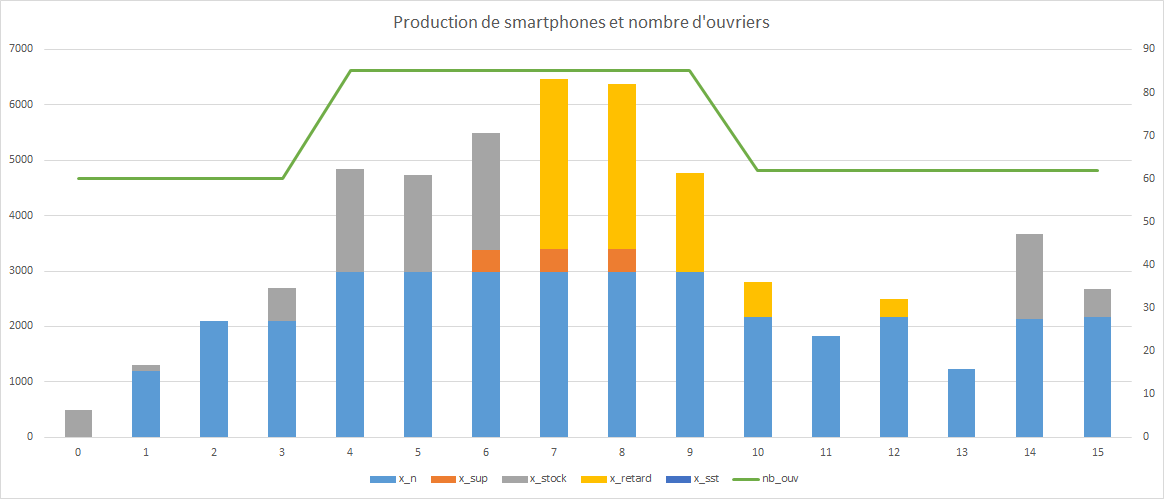
\includegraphics[scale = 0.8]{img/grapheProductionOuv.png}
	  \caption{Répartition du moyen de production des smartphones en fonction des semaines et évolution du nombre d'ouvriers dans le cas entier.}
	  \label{fig:grapheProductionOuv}
  \end{center}
\end{figure}